\newpage
\section{LoRaWAN}
\label{section:lorawan}
LoRaWAN je protokol koji definira kontrolu pristupa komunikacijskom mediju (eng. MAC - Media Access Control) i standard za stvaranje LPWAN mreža baziranih na LoRa tehnologiji.
LoRaWAN definira komunikacijski protokol i arhitekturu mreže oslanjajući se na LoRa tehnologiju obrađenu u poglavlju \ref{section:lora_phy}. Sam protokol i arhitektura mreže imaju izravan utjecaj na trajanje baterije krajnjih uređaja, kapacitet mreže, kvalitetu usluge, sigurnost i druge aspekte bitne za krajnje aplikacije odnosno korisnike LoRa i LoRaWAN tehnologije.
LoRaWAN je dizajnirana primarno za bežične senzorske mreže, ali i druge primjene imajući na umu nekoliko ključnih faktora:
\begin{itemize}
\item Slanje male količine podataka s pojedinog krajnjeg uređaja (čvora)
\item Mala brzina slanja podataka
\item Mala potrošnja energije
\item Kratak period aktivnosti krajnjih uređaja (melen Duty Cycle) - nekoliko poruka dnevno
\item Iznimno velik broj uređaja u mreži - podržava do 1 milijun uređaja
\item Podrška za razne načine rada uređaja - mogučnost optimiranja potrošnje
\item Sigurnost
\end{itemize}
Iako LoRa modulacijski postupak nije otvoreno rješenje, LoRaWAN je otvoreni standard kojeg specificira neprofitna \href{https://lora-alliance.org}{LoRa alijansa}. Glavna zadaća svih članova LoRa alijanse je suradnja na razvoju LoRaWAN standarda. Aktualna verzija LoRaWAN specifikacije je \href{https://lora-alliance.org/resource-hub/lorawantm-specification-v11}{1.1}
\newline

Bitno je napomenuti da je moguće koristiti LoRa tehnologiju i bez LoRaWAN protokola. Međutim, LoRaWAN je široko prihvaćen otvoreni standard i takva situacija nije česta. Na primjer, možemo koristiti LoRu bez LoRaWAN protokola kada želimo ostvariti vezu između samo dva LoRa primopredajnika (peer-to-peer).
        
\subsection{Arhitektura mreže}
\label{subsection:lorawan_network_arh}
LoRaWAN koristi zvijezdastu topologiju mreže. Svaki krajnji uređaj u mreži može komunicirati (bidirekcionalno) sa više LoRa premosnika (eng. LoRa gateway). Dakle, krajnji uređaj nema definiran vlastiti premosnik već se okviri šalju svim premosnicima (eng. Broadcast). S obzirom da u mreži može biti više premosnika povezanih na mrežni server, a sa svakim premosnikom može biti povezano više krajnjih uređaja, često se kaže da LoRaWAN ima dvostruku zvijezdastu topologiju (eng. Star of Stars).
\begin{figure}[ht!]
	\centering
	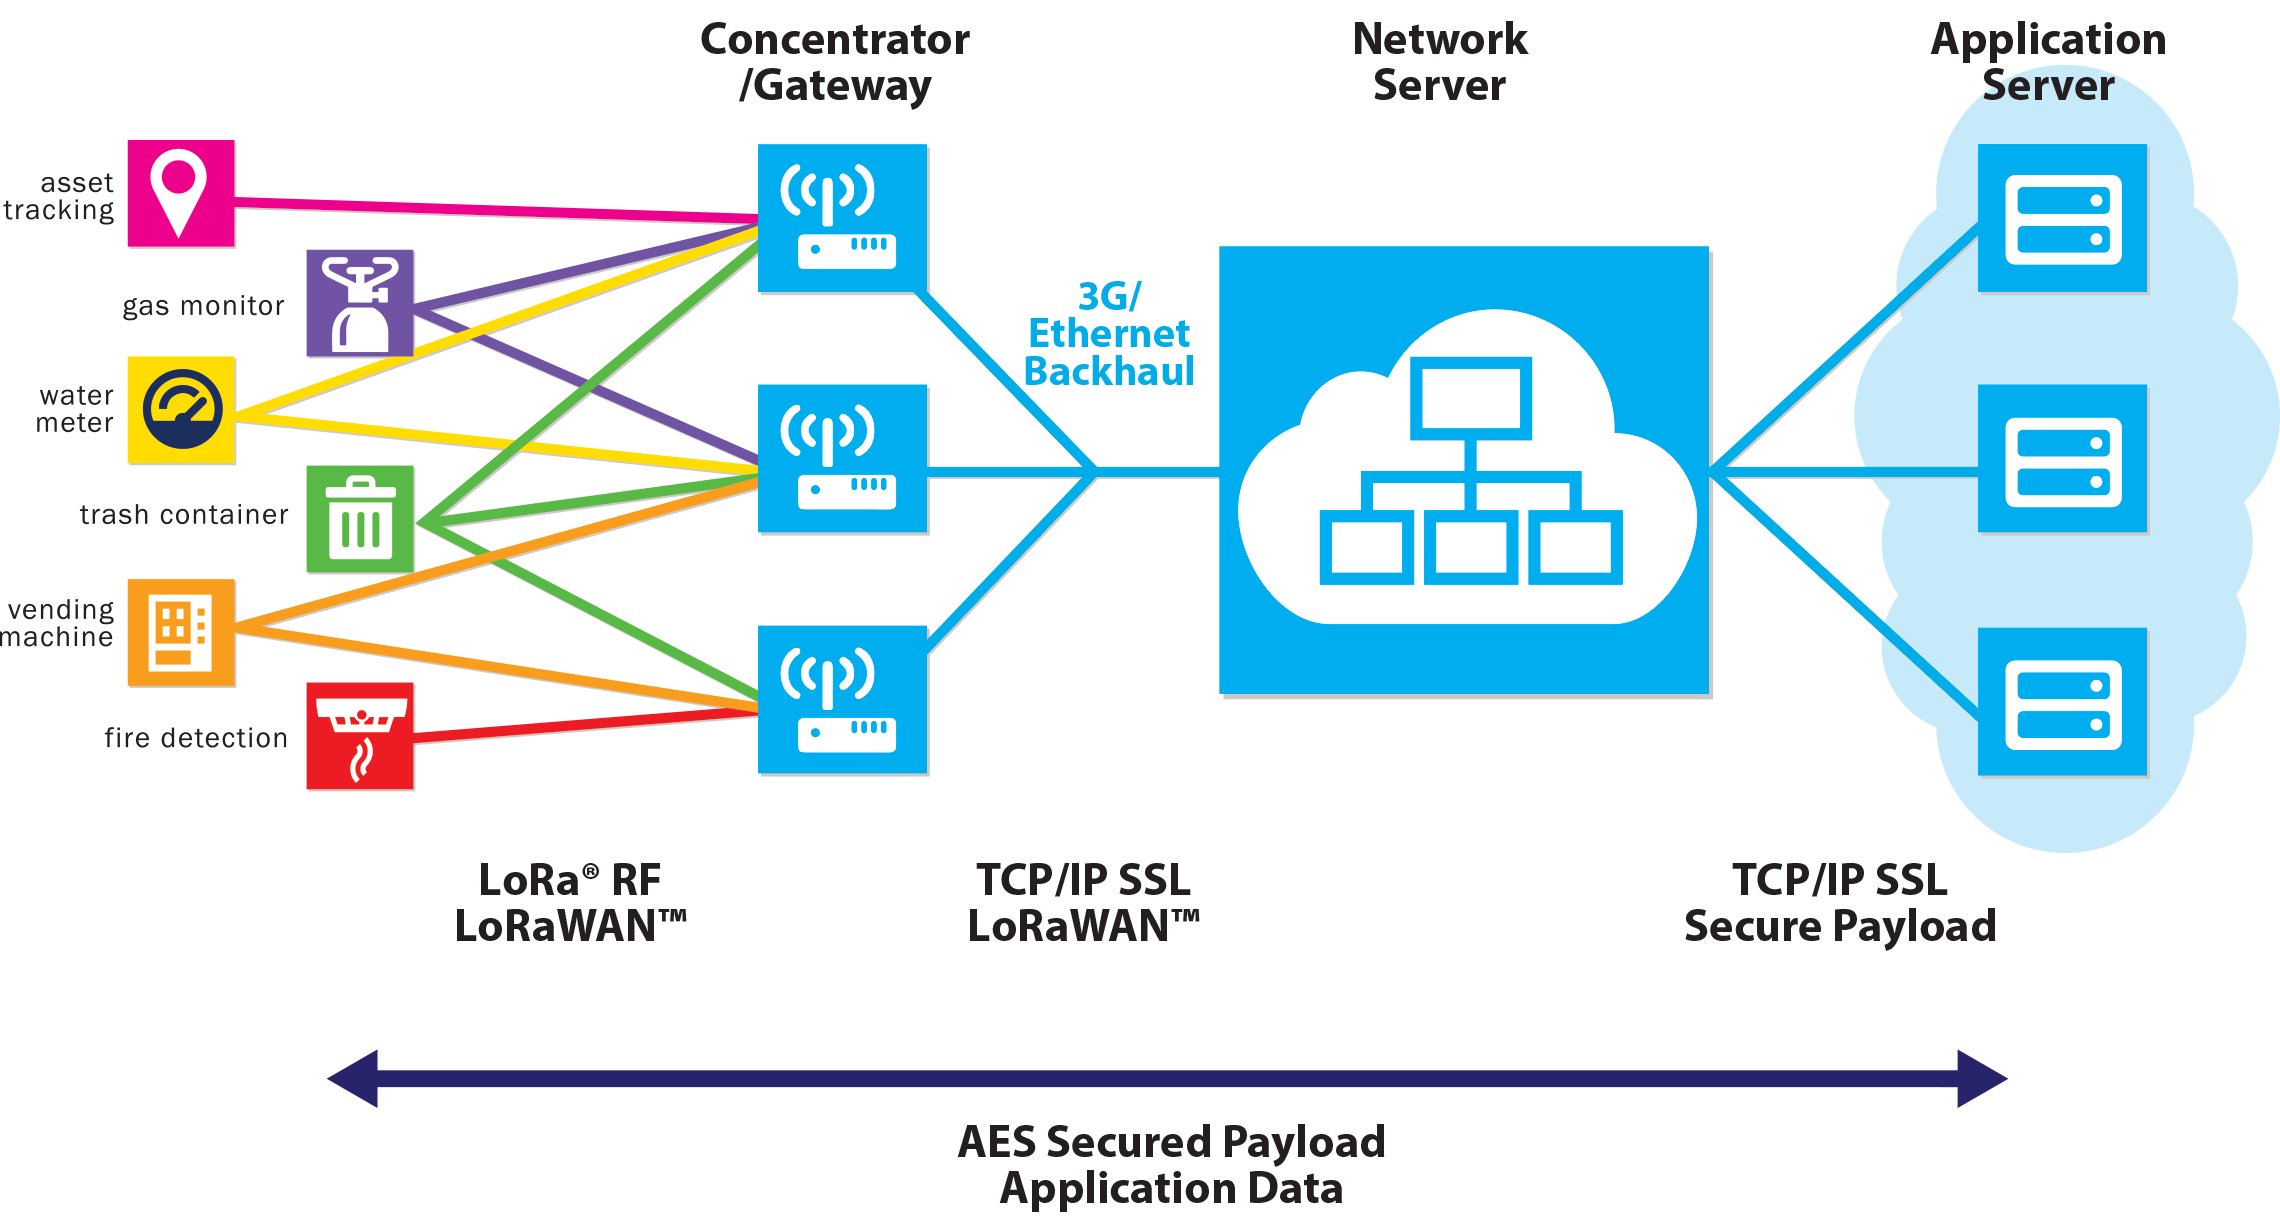
\includegraphics[width=1.0\textwidth]{images/lorawan_network.png}
	\caption{Topologija LoRaWAN mreže}
	\label{img:bands}
\end{figure}

\subsection{Komponente LoRaWAN mreže}
\label{subsection:lorawan_components}
LoRaWAN specifikacija definira nekoliko komponenti potrebnih za ostvarenje LoRaWAN mreže:
\begin{itemize}
\item \textbf{Krajnji LoRa uređaj} - uređaj male potrošnje električne energije, opremljen senzorima i/ili aktuatorima, komunicira s premosnicima

\item \textbf{LoRa premosnik} (eng. Gateway) - prosljeđuje pakete primljene od krajnjih uređaja prema mrežnom poslužitelju i obrnuto. Komunikacijsko sučelje prema krajnjim uređajima je LoRa, a prema mrežnom poslužitelju IP (npr. Ethernet ili 4G) što omogućuje veliku propusnost prema mrežnom poslužitelju koja je nužna zbog velikog broja krajnjih uređaja. Više premosnika može primiti isti paket, ali ga svi prosljeđuju prema mrežnom poslužitelju. Premosnik dodaje podatke o kvaliteti signala. Premosnik se također brine o vremenskim intervalima unutar kojih se paketi šalju prema krajnjim uređajima tj. brine se o sinkronizaciji s krajnjim uređajima.

\item \textbf{LoRa mrežni poslužitelj} - ostvaruje stalnu vezu s premosnicima i prosljeđuje poruke odgovarajućim aplikacijskim poslužiteljima. Obavlja agregaciju primljenih paketa i odbacuje duplikate primljenih paketa. Stvara ACK poruku za poruke koje zahtjevaju potvrdu. Zaprima poruke od aplikacija, generira pakete koji se šalju prema krajnjim uređajima i prosljeđuje ih premosnicima. Odlučuje koji će premosnik odgovoriti krajnjem uređaju tako što prati parametre komunikacije odnosno kvalitetu pojedine veze u mreži (eng. RSSI - Received Signal Strength Indication). Mrežni poslužitelj upravlja mrežom i krajnjim uređajima slanjem MAC naredbi. Možemo reći da je kompleksnost LoRaWAN protokola najvećim dijelom sadržana u mrežnom poslužitelju što je i logično ako se želi uštediti energija na krajnjim uređajima.

\item \textbf{Aplikacijski poslužitelj} - prikuplja i analizira podatke i šalje poruke prema krajnjim uređajima preko ostatka mreže. Ujedno veza između korisničke aplikacije i LoRa poslužitelja.
\end{itemize}

\subsection{Klase uređaja}
\label{subection:classes}
LoRaWAN specifikacija definira tri klase krajnjih uređaja odnosno tri načina rada. Svi krajnji uređaji moraju implementirati klasu A, a klasa B i C su proširenja na specifikaciju klase A.
\begin{itemize}
\item \textbf{Klasa A} - energetski najštedljivija, ograničeno bi-direkcionalna (nepoznata latencija)

U klasi A komunikaciju uvijek iniciraju krajni uređaji i potpuno je asinkrona. Komunikacija od krajnjih uređaja prema premosnicima može biti pokrenuta u bilo kojem trenutku. Nakon uplink komunikacije slijede, s vremenskim odmakom (RxDelay), 2 prozora (RX1 i RX2) unutar kojih se može odviti downlink komunikacija tj. slanje prema krajnjim uređajima. Poruke sa poslužitelja u bilo kojem drugom trenutku moraju pričekati da krajni uređaj inicira komunikaciju kako bi u idućem downlink prozoru mogli poslati svoje poruke. Drugim riječima downlink komunikacija ovisi o uplink komunikaciji pa je nepoznata downlink latencija, ali ipak postoji mogučnost bi-direkcionalne komunikacije.
\begin{figure}[ht!]
	\centering
	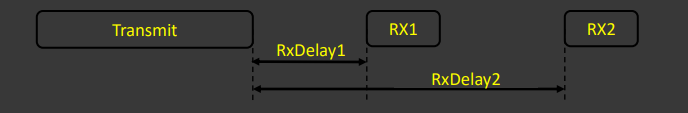
\includegraphics[width=0.9\textwidth]{images/a_class.png}
	\caption{Klasa A}
	\label{img:class_a}
\end{figure}
\newpage
\item \textbf{Klasa B} - bi-direkcionalna komunikacija sa poznatom latencijom, malo veća potrošnja energije

Klasa B je proširenje klase A gdje su uređaji u mreži sinkronizirani tzv. periodičkim \textit{beacon} signalom kojeg postavlja premosnik. U klasi B postoje dodatni downlink prozori (tzv. ping slot) u periodičkim trenucima. Premosnici znaju trenutke u kojima krajnji uređaji slušaju te tada mogu obaviti slanje paketa prema krajnjim uređajima. Latencija je deterministička i podesiva do 128 sekundi kako bi se komunikacija mogla prilagoditi raznim aplikacijama, a da se zadrži mala potrošnja energije.
\begin{figure}[ht!]
	\centering
	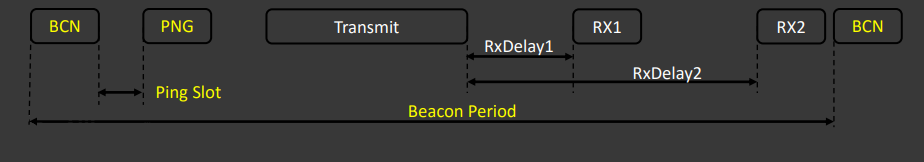
\includegraphics[width=0.9\textwidth]{images/b_class.png}
	\caption{Klasa B}
	\label{img:class_b}
\end{figure}
\item \textbf{Klasa C} - najmanja latencija (praktički Half-Duplex komunikacija), najveća potrošnja energije

Proširenje klase A: nakon uplink komunikacije tj. slanja od krajnjeg uređaja prema premosnicima i isteka vremenskog perioda RxDelay, krajnji uređaj nastavlja slušati sve do slijedećeg slanja prema premosnicima. Nedostatak klase C je iznimno velika potrošnja energije ako ju usporedimo s klasom A i B.

\begin{figure}[ht!]
	\centering
	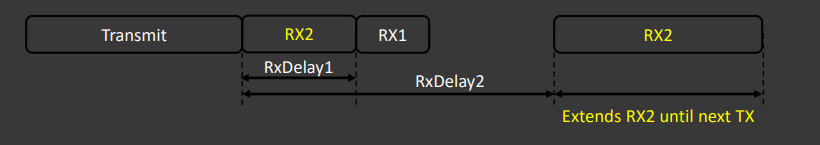
\includegraphics[width=0.9\textwidth]{images/c_class.png}
	\caption{Klasa C}
	\label{img:class_c}
\end{figure}
\end{itemize}

\subsection{Adaptive Data Rate (ADR)}
Kako bi se maksimiziralo trajanje baterije krajnjih uređaja i kapacitet mreže, a ostvarila potrebna brzina i doseg komunikacije, LoRaWAN mrežni poslužitelj upravlja postavkom DR (Data Rate) i izračenom RF snagom krajnjih uređaja. Postavka DR je izravno povezana s parametrima SF i BW. LoRa premosnici optimiraju mrežu tako što iskorištavaju svojstvo da na istom frekvencijskom rasponu BW mogu istovremeno primati podatke ako oni dolaze drugačijim parametrom SF (pogledati potpoglavlje o virtualnim kanalima \ref{subsection:lora_virt_channel}). Brzine prijenosa u LoRaWAN mreži variraju između nekoliko bps do 50kbps za isti parametar BW.

\subsection{Kapacitet mreže}
Visok kapacitet mreže potreban je zbog velikog broja krajnjih uređaja koji komuniciraju s premosnicima. Kapacitet mreže ključna je osobina mreže bitna za performanse i skalabilnost same mreže. Visok kapacitet u LoRaWAN mreži je osim podesivim parametrom DR ostvaren i višestrukim komunikacijskim kanalima.
\begin{figure}[ht!]
	\centering
	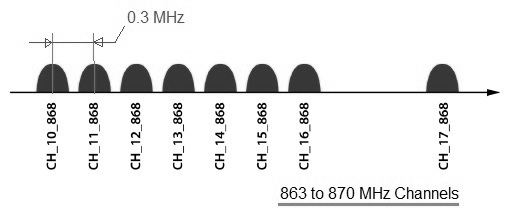
\includegraphics[width=0.9\textwidth]{images/lora_channels.jpg}
	\caption{Kanali LoRa 868MHz spektra (EU)}
	\label{img:channels}
\end{figure}
LoRa premosnici su dizajnirani tako da istovremeno mogu primati poruke na više kanala (eng. Multichannel i Multimodem), a još k tome na svakom fizičkom kanalu postoje virtualni kanali što efektivno dodatno povečava kapacitet mreže.

\subsection{Format LoRaWAN poruke}
\label{subsection:lorawan_packet}
LoRaWAN poruka se enkapsulira u LoRa fizički okvir opisan u potpoglavlju \ref{subsection:lora_frame}. Format LoRaWAN paketa prikazan je na slijedećoj slici.
\begin{figure}[ht!]
	\centering
	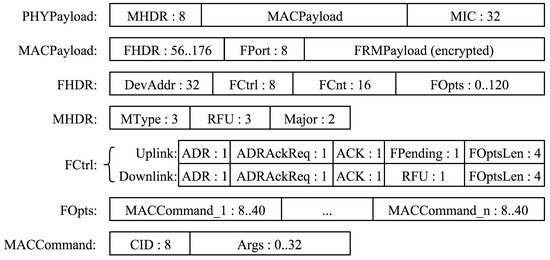
\includegraphics[width=0.9\textwidth]{images/packet.jpg}
	\caption{LoRaWAN paket}
	\label{img:lorawan_packet}
\end{figure}

\newpage
Polja LoRaWAN poruke:
\begin{itemize}
\item MHDR (MAC header) - definira tip poruke
\item MACPayload - podaci LoRaWAN poruke (sastoji se od zaglavlja okvira(FHDR), podataka okvira (FRMPayload) i porta FPort)
\item MIC (Message Integrity Code) - osigurava integritet poruke
\item DevAddr - kratka adresa uređaja
\item FPort - ako je vrijednost 0, radi se o MAC naredbi
\item FRMPayload - korisni podaci okvira kriptirani 128 bitnim AES ključem
\item FCtrl - kontrolni oktet
\begin{itemize}
\item FOptsLen - duljina FOpts polja - 0 ako se radi o MAC naredbi
\item vrsta poruke (uplink ili downlink)
\item ACK - zahtjev za potvrdom
\item ADR - podesivi Data Rate
\item FPending - oznaka da postoji još podataka za slanje (samo u downlink porukama)
\end{itemize} 
\item FCnt - brojač okvira
\item FOpts služi za prijenos MAC naredbi  u podatkovnoj poruci, ako postoji, polje FOpts je kriptirano NwkSEncKey ključem (ključem enkripcije na razini mreže).
\end{itemize}

\subsection{Integriranje krajnjeg uređaja u LoRaWAN mrežu}
\label{subsection:end_node_integration}
Kako bi sudjelovao u LoRaWAN mreži, krajnji uređaj mora biti aktiviran. Dostupna su dva načina aktivacije krajnjih uređaja: OTAA (Over-The-Air Activation) i ABP (Activation By Personalization):
\begin{itemize}
\item OTTA - Procedura aktivacije kod koje se koriste zahtjevi za pristup (eng. join-request) i odgovori na zahtjeve za pristup (eng. join-accept) mreži. Ovisno o odgovoru na zathjev, krajnji uređaj mogu dobiti ključeve za novu mrežnu i aplikacijsku sesiju.
\item ABP - ključevi za sesiju su izravno upisani u krajnje uređaje
\end{itemize}
Svakom krajnjem uređaju potrebne su slijedeće informacije kako bi se mogao integrirati u mrežu:
\begin{itemize}
\item Adresa krajnjeg uređaja (DevAddr) - 32-bitni identifikator krajnjeg uređaja, 7 bitova je identifikator mreže, a preostali identifikator uređaja
\item Identifikator AppEUI - globalni identifikator iz IEEE EUI64 adresnog prostora koji jedinstveno identificira krajnji uređaj
\item Ključ mrežne sesije (NwkSKey) - ključ korišten od strane mrežnog poslužitelja i krajnjeg uređaja u svrhu verficiranja integriteta poruke i autentifikacije uređaja
\item Ključ aplikacijske sesije (AppSKey) - ključ korišten od strane mrežnog poslužitelja i krajnjeg uređaja u svrhu kriptiranja i dekriptiranja korisnih podataka u poruci
\end{itemize}

\subsection{Sigurnost}
\label{subsection:security}
Iznimno je bitno za svaku LPWAN mrežu pa tako i za LoRaWAN da implementira sigurnost.
LoraWAN protokol sadrži sigurnost u dva sloja: jedan sloj sigurnosti za mrežu (NwkSKey ključ) i jedan sloj za aplikaciju (AppSKey ključ). Mrežni sloj sigurnosti se brine za autentifikaciju kranjeg uređaja (kriptiranjem poruke), a aplikacijski sloj sigurnosti osigurava kontrolu pristupa aplikacijskim podacima (kriptiranjem podataka AES enkripcijom).

\begin{figure}[ht!]
	\centering
	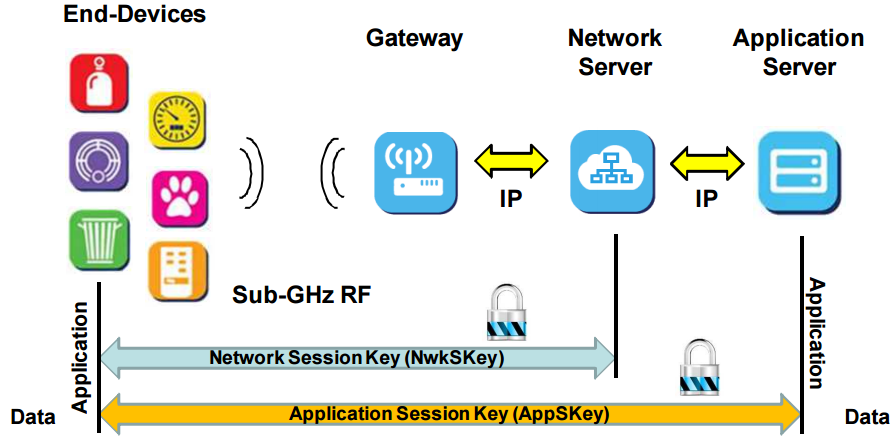
\includegraphics[width=0.9\textwidth]{images/security.png}
	\caption{Slojevitost sigurnosti LoRaWAN protokola}
	\label{img:security}
\end{figure}